\documentclass[obeyFinal]{llncs}
\usepackage{llncsdoc}
\usepackage{fainekos-macros}
\usepackage{color}


\usepackage[english]{babel}
\usepackage{amsmath}
\usepackage{graphicx}
\usepackage[colorinlistoftodos,obeyFinal]{todonotes}
\usepackage{wrapfig}
\usepackage{makeidx}  % allows for indexgeneration
\usepackage{bibspacing}
\usepackage{fancyvrb}
\usepackage{amsfonts}
\usepackage{color}
\usepackage[ruled]{algorithm}
\usepackage{algpseudocode}
\usepackage{authblk}

\setlength{\bibspacing}{\baselineskip}
\usepackage[tight,footnotesize]{subfigure}

\newcommand{\tableref}[1]{Table~\ref{tab:#1}}
\newcommand{\figref}[1]{Fig.~\ref{fig:#1}}
\newboolean{TECH_REPORT}
\newcommand{\process}[1]{{\color{red}\emph{#1}}}
\DeclareSymbolFont{extraup}{U}{zavm}{m}{n}
%\setlength{\textwidth}{12.5cm}
%\setlength{\textheight}{20.4cm}
\usepackage{tikz}
\newcommand*\circled[1]{\tikz[baseline=(char.base)]{
		\node[shape=circle,draw,inner sep=2pt] (char) {#1};}}
\setboolean{TECH_REPORT}{TRUE}
\booltrue{HIGHLIGHTCHANGES}%{true}

\begin{document}
%\title{High confidence verification of medical device software}
\title{The Challenge of High-Confidence Medical Device Software}

\author{Zhihao Jiang, Houssam Abbas, Kuk Jin Jang and Rahul Mangharam}
\institute{Department of Electrical and Systems Engineering, University of Pennsylvania, USA\\
\{zhihaoj, habbas, jangkj, rahulm\}@seas.upenn.edu}


\maketitle
\section{The Promise and Challenges of Medical Devices}
Medical devices play an essential role in the care of patients around the world, and can have a life-saving effect.
To cite one example, 
an estimated 3 million people worldwide have implanted pacemakers (a heart rate adjustment device), with $\sim$600,000 added annually.
%Cardiac Pacemakers From the Patient's Perspective circ.ahajournals.org/content/105/18/2136.full
In the United States, 800,000 people have an implanted defibrillator (another heart rhythm management device), with 10,000 added monthly.
%http://asktheicd.com/tile/106/english-implantable-cardioverter-defibrillator-icd/how-many-people-have-icds/
Clinical trials have presented evidence that patients implanted with defibrillators have a mortality rate reduced by up to 31\%.

% MADIT II trial
The medical device is a \$289 billion market with \$110 billion within the US.
%Of that, , with this number projected to reach \$133 billion in 2016.
%http://selectusa.commerce.gov/industry-snapshots/medical-device-industry-united-states
Examples include everything from adhesive bandages to drug infusion pumps, surgical robots, deep brain stimulation systems and physiological closed-loop control systems like the artificial pancreas~\cite{pancreas_paul} which are in development.
%In fact, many device companies are in the no-revenue startup phase, indicating a vigorous research environment.
These are safety-critical technologies combining hardware and software, each of which must be rigorously verified to be efficacious and safe.

According to the US Food and Drug Administration, in 1996, 10\% of all medical device recalls were caused by software-related issues. 
This percentage rose to an average of 15\% of recalls from 2008 to 2012. Implanted cardiac pacemakers and defibrillators have approximately 80,000-100,000 lines of software code~\cite{pauljones} which essentially makes all sensing, control and actuation decisions autonomously within the human body, over the 5-7 year device lifetime. The primary challenge of high-confidence medical device software is to guarantee the device will never drive the patient into an unsafe condition even though we do not have complete understanding of the physiological plant. 
%The medical device market is worth \$289 billion.
%Of that, \$110 billion is in the US alone, with this number projected to reach \$133 billion in 2016.
%%http://selectusa.commerce.gov/industry-snapshots/medical-device-industry-united-states
%Examples include everything from adhesive bandages to surgical robots, including pacemakers (a heartbeat adjustment device) and devices still undergoing basic research like the artificial pancreas.
%In fact, many device companies are in the no-revenue startup phase, indicating a vigorous research environment.
%To take one example of the societal impact of medical devices, 
%an estimated 3 million people worldwide have implanted pacemakers, with an extra 600,000 added annually.
%%Cardiac Pacemakers From the Patient's Perspective circ.ahajournals.org/content/105/18/2136.full
%Clinical trials have presented evidence that patients implanted with defibrillators (another heart rate adjustment device) have a mortality rate reduced by up to 31\%.
%% MADIT II trial
%These are life-saving technologies combining hardware and software, each of which must be rigorously verified to be efficacious and safe.
%According to the US Food and Drug Administration, in 1996, 10\% of all medical device recalls were caused by software-related issues. 
%This percentage rose to an average of 15\% of recalls from 2008 to 2012. 

\subsection{Human-in-the-loop Medical Devices}
Medical devices can be classified as open-loop or closed-loop.
A \emph{closed-loop device} like a pacemaker is in a feedback loop with the organ(s) it affects (see Fig.\ref{fig:pacemaker}): it monitors certain physiological variables like heart rate, and delivers therapy, in the form of low-energy electrical pulses, to maintain a healthy heart rate.
Another example is the artificial pancreas, which monitors blood glucose levels and delivers therapy, in the form of insulin, to maintain safe glucose levels.
An \emph{open loop device} on the other hand, either, (a) like a drug infusion pump, does not measure any physiological variables: the therapy it delivers is pre-programmed and non-reactive; or (b) as in the case of a blood pressure monitor, only measures physiological signals but does not deliver therapy. 
\begin{figure}[t]
	\centering
	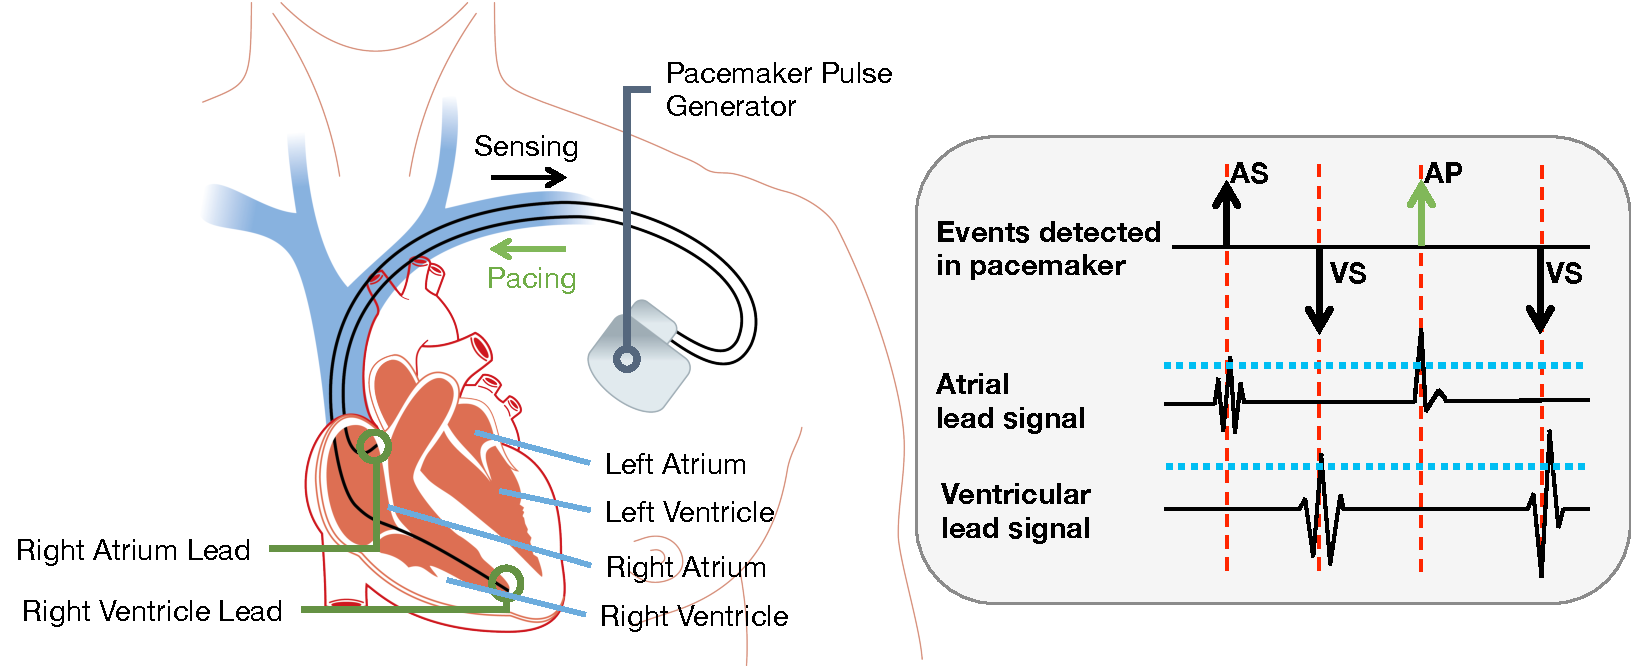
\includegraphics[width=\textwidth]{figs/fig1pacemaker.pdf}
	\caption{\small Pacemaker operating in a closed-loop with the heart. The leads sense cardiac electrophysiological activity from inside the heart tissue (AS/VS = Atrial/Ventricular Sense event) and actuate the heart (AP/VP = Atrial/Ventricular Pacing event} to maintain a desired heart rate.
	\label{fig:pacemaker}
\end{figure}

Open-loop devices are operated by professionals to ensure the safety of the patient.
Closed-loop devices require very little physician intervention after the discharge visit, and hence permit a better lifestyle.
Because they are constantly monitoring the physiological variables, they permit a more timely delivery of therapy. 
The complex run-time diagnoses needed for closed loop performance, and the intricate therapy delivered, has driven most diagnosis and therapy functions into software.
This software is life-critical and verification methods should provide a high confidence in its correctness.

Validating the safety and efficacy of closed-loop software, by definition, requires that the device be connected to the organ(s) it is affecting. 
For example, in the case of a pacemaker, that would be the heart of a living patient.
But with the advent of computer models of physiological functions, such as those encompassed by the Physiome project or presented later in this article, the \emph{model-based design (MBD) of closed-loop medical devices} presents efficient complementary approaches that are actively researched in various disciplines of engineering and computer science.
In MBD, the device (or a model thereof) is connected to a \emph{model} of the ``physiological plant" it interacts with.
By high confidence verification we mean that under all possible behaviors of the physiological models (known or unknown), the device will satisfy its safety properties and not adversely affect the organ.

There are two major differences between modeling physiology and modeling man-made systems:
first, physiology is much more complex and less well-understood than man-made systems like cars and airplanes, and spans several scales from the molecular to the entire human body.
Secondly, the variability between humans is significantly larger than that between two cars coming off the assembly line.
Using the cardiac pacemaker as an example of closed-loop device, and the heart as the organ to be modeled, we present several of the challenges and early results in model-based verification.


\section{Life-critical Closed-loop Software}
\label{sec:eltbroad}

The heart is a specialized muscle that pumps oxygenated blood to the rest of the body.
It is composed of four chambers: two upper chambers called the left and right atrium, and two lower chambers called the left and right ventricle, which contract synchronously.
%The blood depleted of oxygen flows into the right atrium and passes into the right ventricle. 
%The latter contracts and pumps the blood to the lungs.
%Once oxygenated in the lungs, the blood flows into the left atrium and thereafter into the left ventricle. 
%The latter contracts and pumps the oxygenated blood to the rest of the body.
%Ventricular contractions are synchronized, as are atrial contractions.
In a healthy resting adult, the heart rate is 60 to 100 beats per minute (each ventricular contraction is a beat). The contractions of the heart are controlled by the waves of spontaneous electric depolarization that traverse it regularly.
A spontaneous electric current originates in the \emph{Sino-Atrial (SA) node} in the right atrium and propagates throughout the atria, causing them to contract. 
It then propagates down to the ventricles along well-defined conduction pathways, causing the ventricles to contract in turn.
The SA node is thus termed the natural pacemaker of the heart.

Under certain diseased conditions, the heart rate drops below what is needed to maintain adequate blood flow to the body. 
This clinical condition is called \emph{bradycardia}.
When such a heart rate drop is due to abnormalities in the electrical conduction system, an implanted pacemaker might be recommended as treatment. A pacemaker is implanted near the left collar of the patient as shown in Fig.\ref{fig:pacemaker},
and has two leads: one connects to the right atrium, the other to the right ventricle. 

The leads act as both sensors and effectors: if the pacemaker fails to sense electric activity on either lead within certain time constraints, indicative of a delayed/missed contraction, it will send an electric pulse to the corresponding chamber to provoke contraction, thus acting as an artificial pacemaker.
The algorithms for detecting missed beats are complex and implemented in software which runs within the pacemaker itself. 
Part of the difficulty of performing that detection comes from the great variability in heart rates between patients and even within a single patient across time.
Moreover, because the pacemaker is limited to sensing electrical activity through its two leads, different phenomena can manifest themselves identically to the pacemaker, thus making detection even harder.

For example, in Endless Loop Tachycardia (ELT), this ambiguity causes the pacemaker to actually \emph{induce} dangerously elevated heart rates (tachycardia), which would not have arisen had the heart been operating on its own.
This is an example of a \emph{adverse closed-loop condition}: a dangerous situation that arises as a result of the \emph{interaction} between device and heart.
No amount of open-loop device testing and verification can reveal this condition - hence the need for closed-loop validation of medical devices, and for physiological heart models that enable early and affordable closed-loop validation.

\section{Choosing the right model for the job}
\label{sec:rightmodel}

Heart models of different kinds have been developed for a range of applications and 
\figref{models} shows four heart modeling approaches that emphasize the electric, mechanical, cellular and fluid flow mechanisms of cardiac function. 
Several of these modeling approaches employ over 4 million finite elements or 100,000 ordinary differential equations to describe the dynamics and take several hours to simulate a single cardiac cycle. 
%Several models of the heart have been developed and used in different applications. 
%It should be noted that most models are developed by experiments on animal hearts, in particular pigs.

\emph{Cellular models} describe the generation and spread of electrical action potentials (i.e., voltages) at the molecular-cellular level \cite{PullanBC05_ElectricModelingBook}.
At the cellular level, the flow of charged ions into and out of the cardiac cell is responsible for the change in voltage across the cell membrane. 
%%These \emph{ion channels} have been modeled extensively, typically through ordinary differential equations that relate ion concentrations to electrical currents and voltages.
Cellular models of electrical activity are used to study how activity across ion channels affect the relation between electrical and mechanical behaviors of heart tissue, as well as to study drug therapies that affect the ion channels properties. 
%%While most models were built from first physics principles, some, like the Fenton-Karma model, are a mix of first principles and behavioral approximations which have no physiological basis, but give a good approximation of the shape of the cross-membrane voltage. 
%%Such simplified models have the advantage of being easier to analyze and faster to simulate.

\emph{Anatomical models} are developed using imaging technologies like MRI, and seek to re-create detailed anatomical structures like fiber orientations and the distribution and extent of scar tissue. 
These structures affect the heart's operation by determining muscle contraction and modifying the speed and paths of electrical conduction throughout the heart. 
Thus anatomical models provide a foundation for whole heart modeling efforts that we cover next.
They are also used to simulate the effects of certain medical devices like stents and artificial valves. 

\begin{figure}[t]
		\centering
		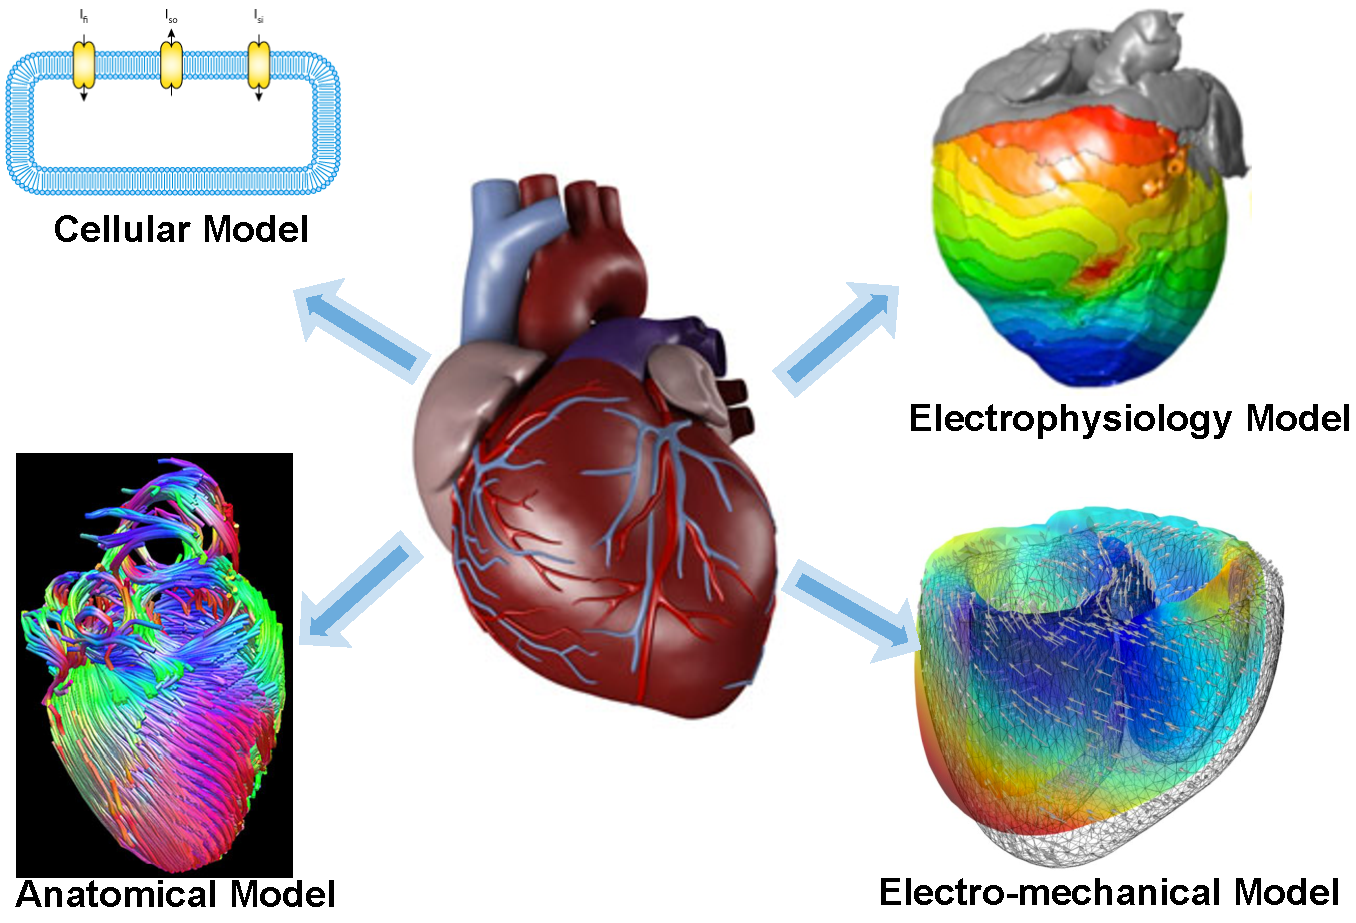
\includegraphics[width=\textwidth]{figs/fig2models.pdf}
		\caption{\small Modelling different phenomena in the heart}
		\label{fig:models}
\end{figure}

\emph{Whole heart models} use a continuum approximation of the cellular models of electrical propagation with the structure obtained from anatomical models. Researchers have developed Partial Differential Equations models of electrical activity in the \emph{whole heart} to analyze the mechanisms of various arrhythmias. 
Researchers at Johns Hopkins \cite{TrayanovaB14_Advances} further used these models to predict the onset of arrhythmias and propose potential therapies. 
Such \emph{electro-mechanical models} help evaluate the mechanical effects of different arrhythmias on blood flow.

\emph{Electrophysiological} (EP) heart models help study the timing properties of the generation and propagation of electrical signals through the electrical conduction system, and can accurately diagnose most arrhythmias. 
%Researchers at Carnegie-Mellon University studied and modeled the heart rate variation
Unlike the aforementioned heart models which are built from the cellular level on up, EP models are developed by conducting a clinical EP testing procedure which is a type or timing analysis of the heart rhythm across the myocardium. EP models are amenable to \emph{model checking}~\cite{model_checking}, a powerful verification technique pioneered in the semiconductor industry.
EP testing is a common method to diagnose arrhythmias: 
a physician inserts catheters with electrodes into the patient's heart through the veins and measures the local electrical activity around the electrodes. 
The physician uses the \emph{patterns} of electrical activity and its timing characteristics to diagnose the heart's condition in terms of arrhythmias, which are derangements to normal timing patterns. 
In particular, electrical timing parameters of action potentials in a tissue region like conduction delay, rest period and refractory period are measured, and any abnormal conduction paths are detected.
%The EP testing studies the timing properties of the generation and propagation of electrical signals through the electrical conduction system, and can accurately diagnose and even treat most arrhythmia. 
\begin{figure}[t]
	\centering
	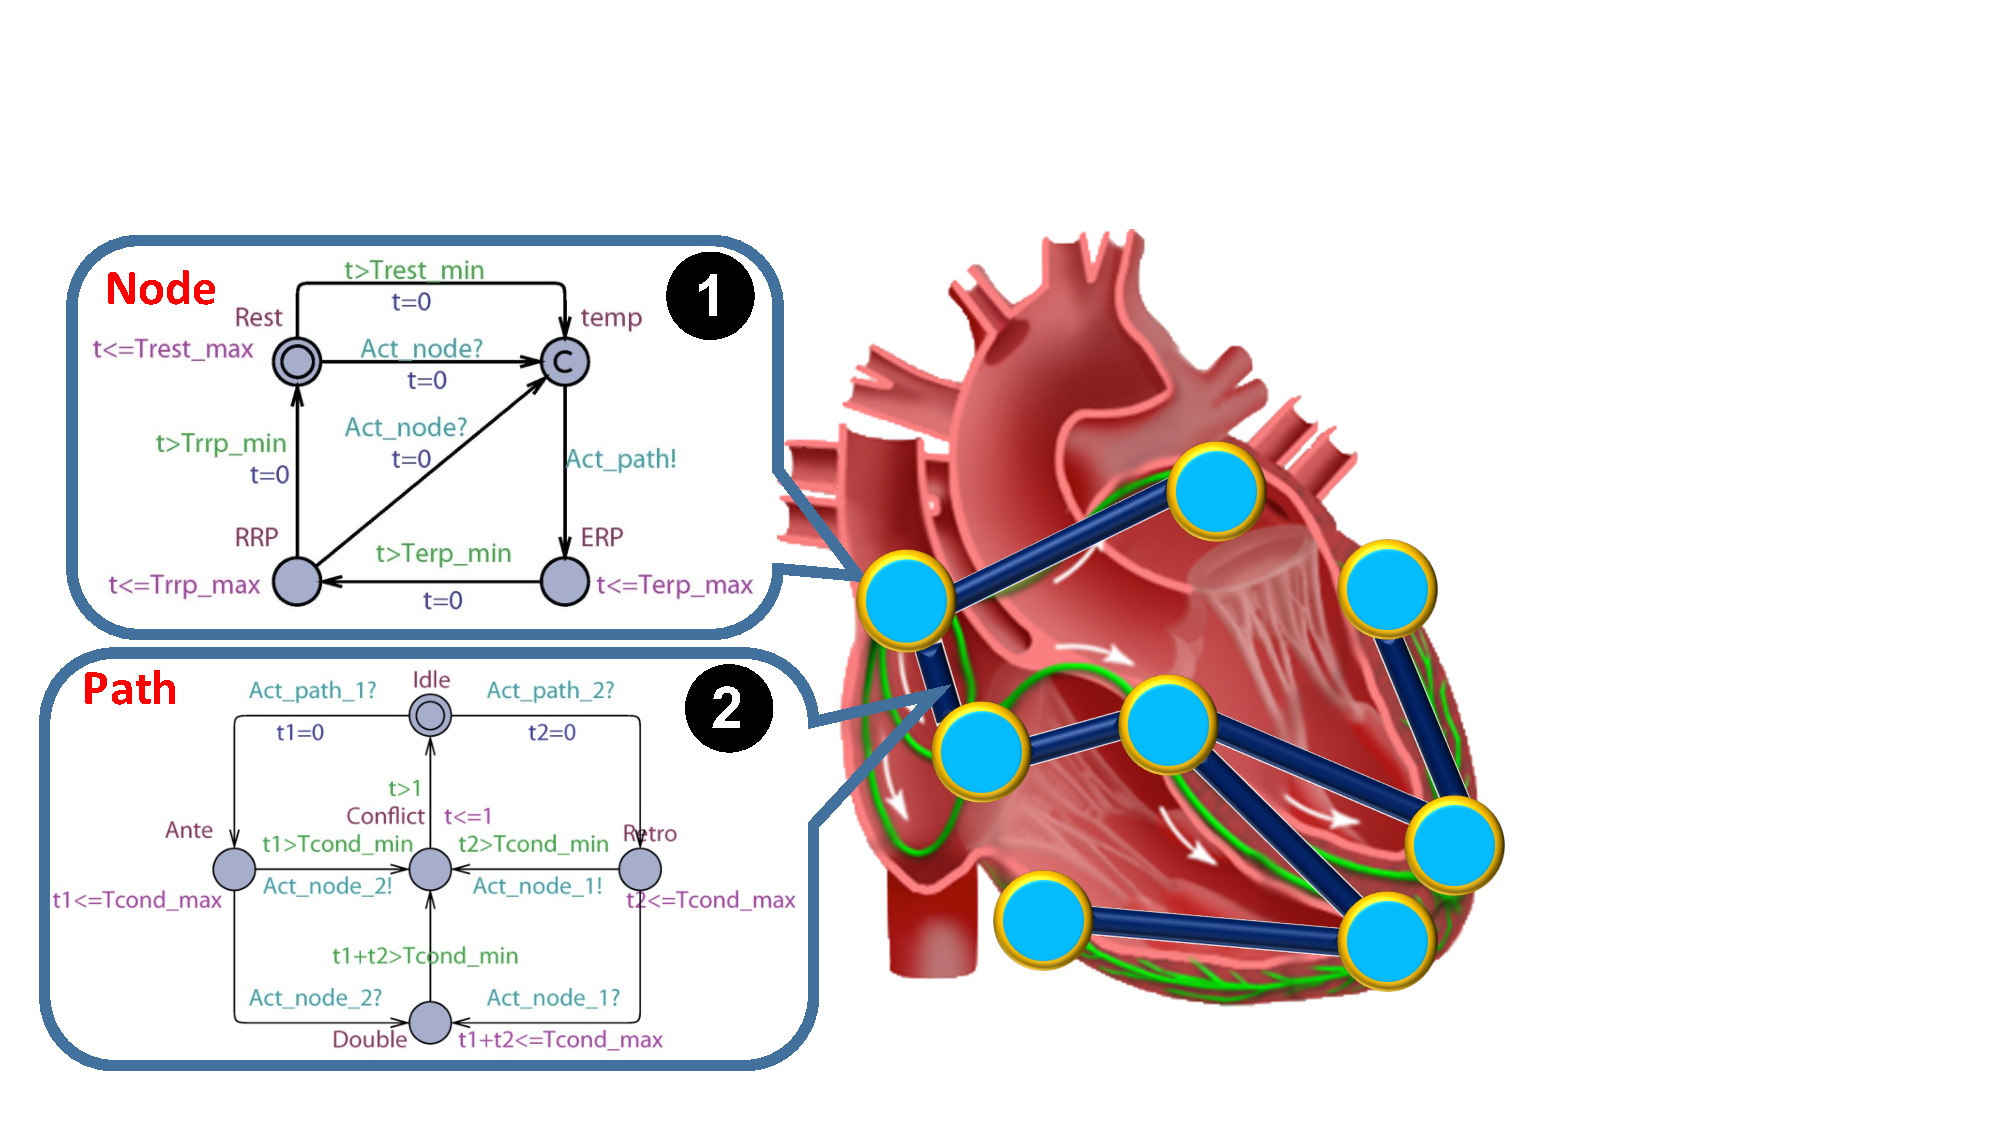
\includegraphics[width=\textwidth]{figs/Pacemaker.pdf}
	\caption{\small Timing of electrical behaviors of the heart are modeled by a network of (1) node and (2) path automata. Each circle is a node automaton which models the generation and blocking of electrical events. Each line is a path automata which models conduction delays between nodes.}
	\label{fig:EP}
\end{figure} 

In \cite{VHM_proc}, researchers from the University of Pennsylvania developed a heart model based on clinical EP testing. 
Since the pacemaker only looks at the \emph{timing} of events as input from only two locations of the heart, this EP model only seeks to model the correct timing of electrical activity in select tissue of the heart.
Specialized tissue like the SA node generates electric events spontaneously and is modeled by Timed Automata known as \emph{node automaton} as shown at Marker 1 in \figref{EP}.
The node automaton models the timing of signal generation, blocking and transmission in heart structures like the AV node. 
The rest of the tissue is abstracted as variable conduction delays as \emph{path automata} between node automata (Marker 2 in \figref{EP}).
Different heart conditions can be modeled by a network of of node/path automata with different  topologies and parameters (\figref{EP}).
Moreover, pacing applied to the heart can be represented as an external activation signal to the node automata.
EP models have been validated by physicians, and have been used for model checking pacemaker software. 

Finally, data-driven models such as~\cite{Bogdan12_fractional} fit (fractional) differential equations directly to measured heart rate without modeling the underlying mechanisms, and are used for optimal control.

\section{Closed-loop model checking of device software}
Short of clinical trials (which we cover later in this article), current validation practice for closed-loop medical devices focuses on open-loop testing and reviews of the design process.
In such open-loop testing, a set of input sequences is fed to the device, and the device's output is checked for correctness, typically by comparing it to a pre-defined expected output.
Such testing does not evaluate the effect of the device on the organ: e.g., we can't test how the heart rate changes following a pacing by the pacemaker.
Thus, we need a heart model that can interact with the device. 
If we use, say, a high-fidelity PDE-based model such as the electro-mechanical models described earlier to react to the device and generate input sequences, there are an infinite number of heart rhythms that such a model can generate, and testing only uses a finite subset of those.
Thus, testing (whether open-loop or closed-loop with a heart model) is necessarily an incomplete technique, and safety violations of the device may be missed during testing.

The timed automata-based EP models are amenable to \emph{model checking}, a technique that mathematically explores \emph{all} possible executions of the heart model and device software combination against specified requirements (e.g. the pacemaker will not pace the heart beyond an upper rate limit). 
Model checking is widely used in the semiconductor industry to verify chip designs at various levels of abstraction, in particular at the Register Transfer Level (RTL).
Violations of the requirements are returned by the model checking tool as an execution trace, which can be analyzed and used to improve the system. 
To capture the variability in the heart's behavior (more generally, in the physiological phenomena of interest), the heart model is \emph{non-deterministic}: for example, rather than specifying that the conduction delay in the AV node is always 0.14ms, we allow it to be any value in the correct physiological range [0.12, 0.2] ms.
The model checker will \emph{symbolically} explore all executions corresponding to all values in this range (rather than select a few) in search for requirements violations. Subtle errors in the design of safety-critical systems that often elude conventional simulation and testing techniques can be (and have been) found in this way. Because it has been proven cost-effective and integrates well with conventional design methods, model checking has been adopted as a standard procedure for the quality assurance of  automotive and avionics systems, but has yet to enter the world of medical devices.

Endless Loop Tachycardia (ELT) is one example of a safety hazard that arises in the interaction between pacemaker and heart, shown in \figref{ambiguity}.
The ELT starts with an early ventricular contraction (PVC), which is a common scenario even in a healthy person. 
The electrical signal travels from the ventricle to the atrium (red arrows in \figref{ambiguity}), triggering an atrial sense (AS), i.e. the pacemaker senses an event in the right atrium. 
As a result, the pacemaker paces the ventricle (VP) after a pre-programed delay (AVI), which triggers ventricle to atrium conduction again and this VP $\rightarrow$ AS $\rightarrow$ VP positive feedback loop persists. 
The ventricular rate during ELT is determined by the conduction delay from the ventricle to the atrium and the programed delay in the pacemaker, which is very fast.
The healthy condition in \figref{ambiguity} demonstrates the same input-output sequence as ELT. 
In it, the pacemaker paces the ventricle after each atrial event (AS) generated by the SA node (as opposed to an AS conducted from the ventricle as in ELT).
This is correct pacing at an appropriate (and relatively much slower) rate than ELT, and consequently maintains adequate blood flow. 
Failing to distinguish these two conditions in the heart model may introduce false-positive when checking whether ELT exists, i.e. the healthy case returned as evidence for ELT.
%The heart model should be able to distinguish these two conditions to assess the pacemaker's ELT elimination capabilities so that they do not affect other healthy heart functions, which would be otherwise a false-positive.

\begin{figure}[t]
	\centering
	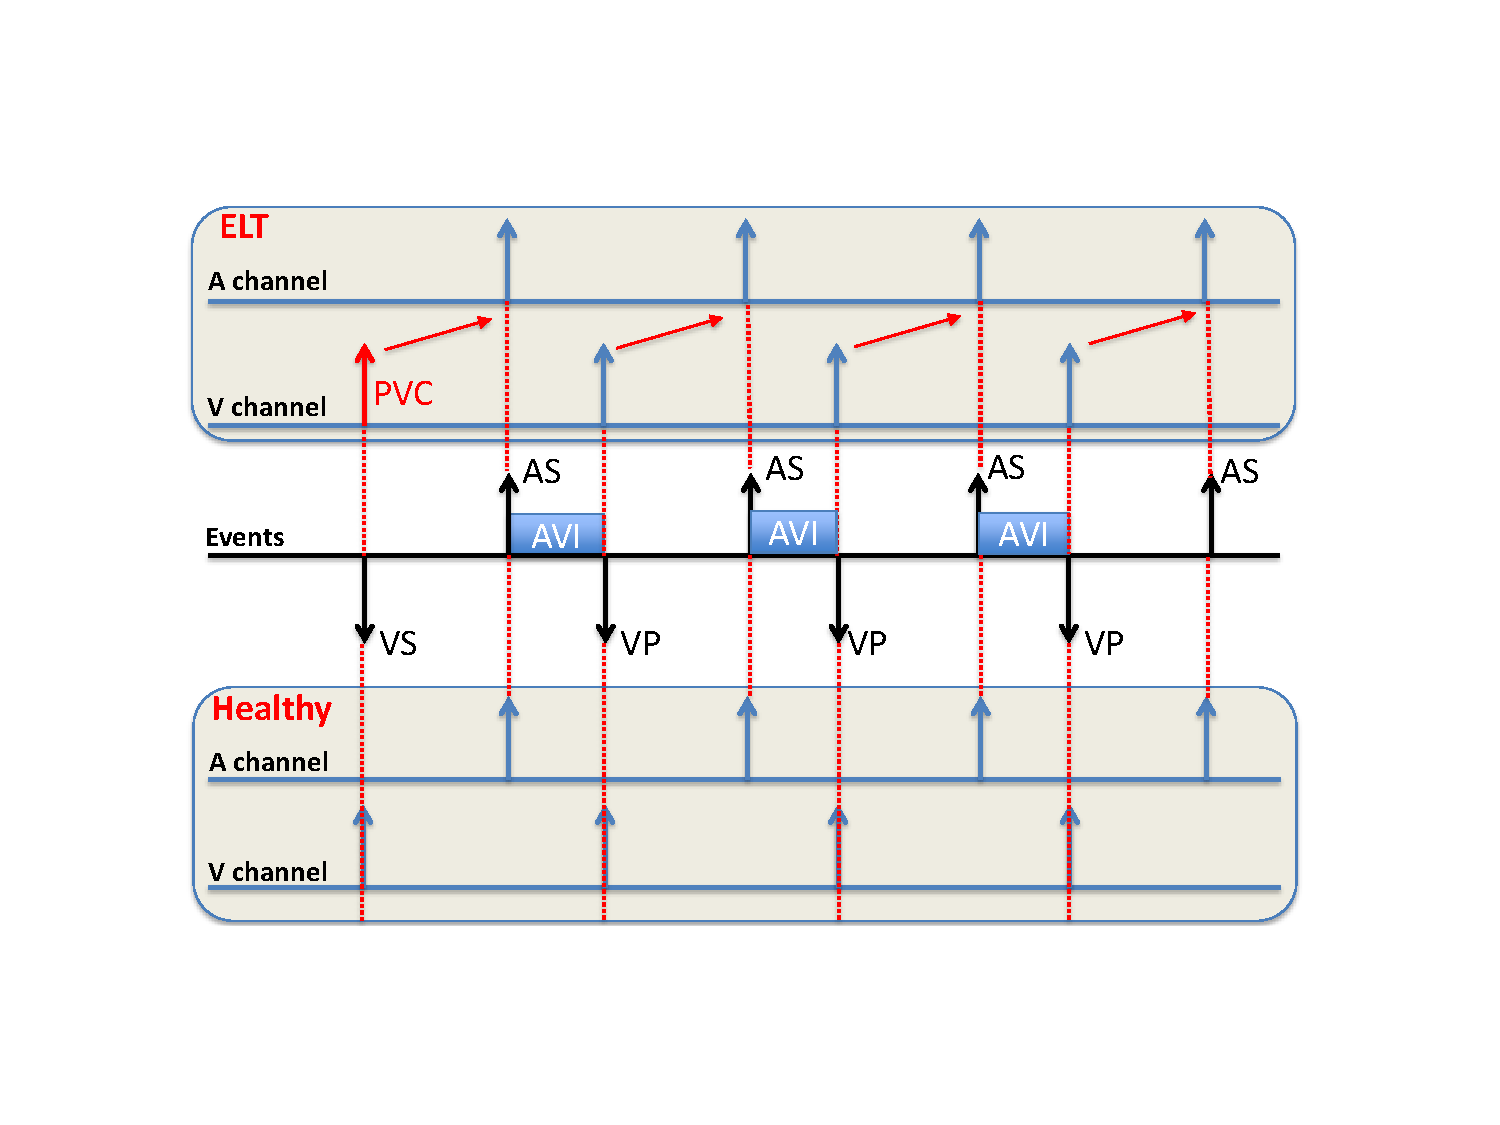
\includegraphics[width=\textwidth]{figs/ambiguity.pdf}
	\caption{\small Endless-loop Tachycardia (ELT) and a healthy heart condition mapped to the same input-output execution of the pacemaker (middle sequence). The heart model should have the details to resolve this ambiguity.}
	\label{fig:ambiguity}
\end{figure}
% \yhl{The heart model should be able to distinguish these two conditions so that an ELT elimination algorithm}
%From the example above, we can see that in order to perform model checking on the closed-loop system, the heart model should not only cover all possible inputs to the pacemaker specified in the requirement, but also have enough details to resolve ambiguities of executions
%% that may introduce false-positives and false-negatives. 
%\figref{abs_tree} demonstrates a collection of heart conditions modeled by the EP heart models. 
%These models are definitely not exhaustive. 
%Model checking the pacemaker model with all these heart models will not guarantee absolute safety. 
%By using physiological abstraction rules (R1-R7 in \figref{abs_tree}), the heart conditions can be generalized and expand the possible inputs to the pacemaker. 
%The result is a heart model $H_{all}$ with only two node automata correspond to the inputs to the pacemaker. 
%By allowing both node automata to be able to send inputs to the pacemaker $[0,\infty]$msec after the last input, the heart model $H_{all}$ covers all possible inputs to the pacemaker. However, $H_{all}$ cannot distinguish the ELT condition from the healthy condition due to the lack of representation of ventricle to atrium conduction. 
%The heart model $H_{cond}$ models the conduction between the atrium and the ventricle with a path automata, thus is the appropriate heart model to evaluate ELT.
\section{Physiological Model Abstraction and Refinement}
%\todo[inline]{I would change the title. Multi-scale is not precise enough, and in hte context of biological modeling, might be understood as cellular to tissue to whole organ modeling - which isnt what this section describes. Perhaps use something more precise like "Modeling abstractions" or "Model Abstraction tree"}
From the example above, we can see that in order to perform model checking on the closed-loop system, the heart model should not only cover all possible inputs to the pacemaker specified in the requirements, but also have enough details to resolve ambiguities of executions that may introduce false-positives and/or false-negatives. 
 The left column of \figref{abs_tree} shows a collection of heart models each modeling a particular heart condition.  
However, these models do not cover \emph{all} possible heart conditions, thus model checking the pacemaker with each of these heart models will not guarantee absolute safety. 
%\figref{abs_tree} shows a collection of heart conditions modeled by the EP heart models. 
%These models do not cover all possible heart conditions, so model checking the pacemaker model with each of these heart models will not guarantee absolute safety. 
%\todo[inline]{The following sentence is ambiguous..."generalized", "expand", it's not clear what you mean. I suggest replacing it with ""}
Physiological abstraction rules (R1-R7 in \figref{abs_tree}) are defined to increase the behaviors of the original model(s), while guaranteeing new behaviors introduced can still be physiologically valid.
%By using physiological abstraction rules , the heart conditions can be generalized and expand the possible inputs to the pacemaker. 
As an example, abstraction rule R4 merges parameter ranges for heart models with the same node and path topologies.
Imagine two node automata $N1,N2$ can self-activate within [300,400]msec and [500,600]msec, respectively.
By applying R4, the new node automaton $N3$ can self-activate within [300,600]msec.
$N3$ covers all behaviors of $N1,N2$, plus new behaviors which are mostly physiologically valid.
If the physiologically-invalid behaviors introduced into $N3$ are returned by the model checker as evidence, they can be eliminated by refining $N3$ back to $N1,N2$.
%\todo[inline]{ZJ: I know it sounds sketchy, but how can we explain the whole idea of abstraction tree with several sentences?}
	%\todo[inline]{instead of a generic example, use actual parameter ranges for actual parameters. E.g. "For example, the rest period of one model being [300,320]ms, and for another model being [400,500]ms, rule R4 replaces these two models by a model whose rest period is the union [300,500]ms. }
%The new abstract model includes all behaviors of the merged heart models, plus new behaviors that may or may not be physiologically valid.}\todo[inline]{confusing, because we don't give a consequence of this. so what if they're not valid? how do we know if they're valid? Not valid sounds bad, is it? what point are we making? I suggest sticking to the example}.

By systematically applying the abstraction rules on the initial set of heart models, we get an abstraction tree  (\figref{abs_tree}) .
The root of the abstraction tree is a heart model $H_{all}$ with only two node automata corresponding to the inputs to the pacemaker.
By allowing both node automata to be able to send inputs to the pacemaker $[0,\infty]$msec after the last input, the heart model $H_{all}$ covers all possible inputs to the pacemaker. However, $H_{all}$ cannot distinguish the ELT condition from the healthy condition due to the lack of representation of ventricle to atrium conduction. 
The heart model $H_{cond}$ (\figref{abs_tree}) models the electrical conduction between the atria and the ventricles with a path automaton, thus is the appropriate heart model to evaluate ELT. 
Similarly, more complex properties will lead to appropriately detailed models along the Model Abstraction Tree.%\todo{first time you mention abstraction tree...}

\begin{figure}[t]
	\centering
	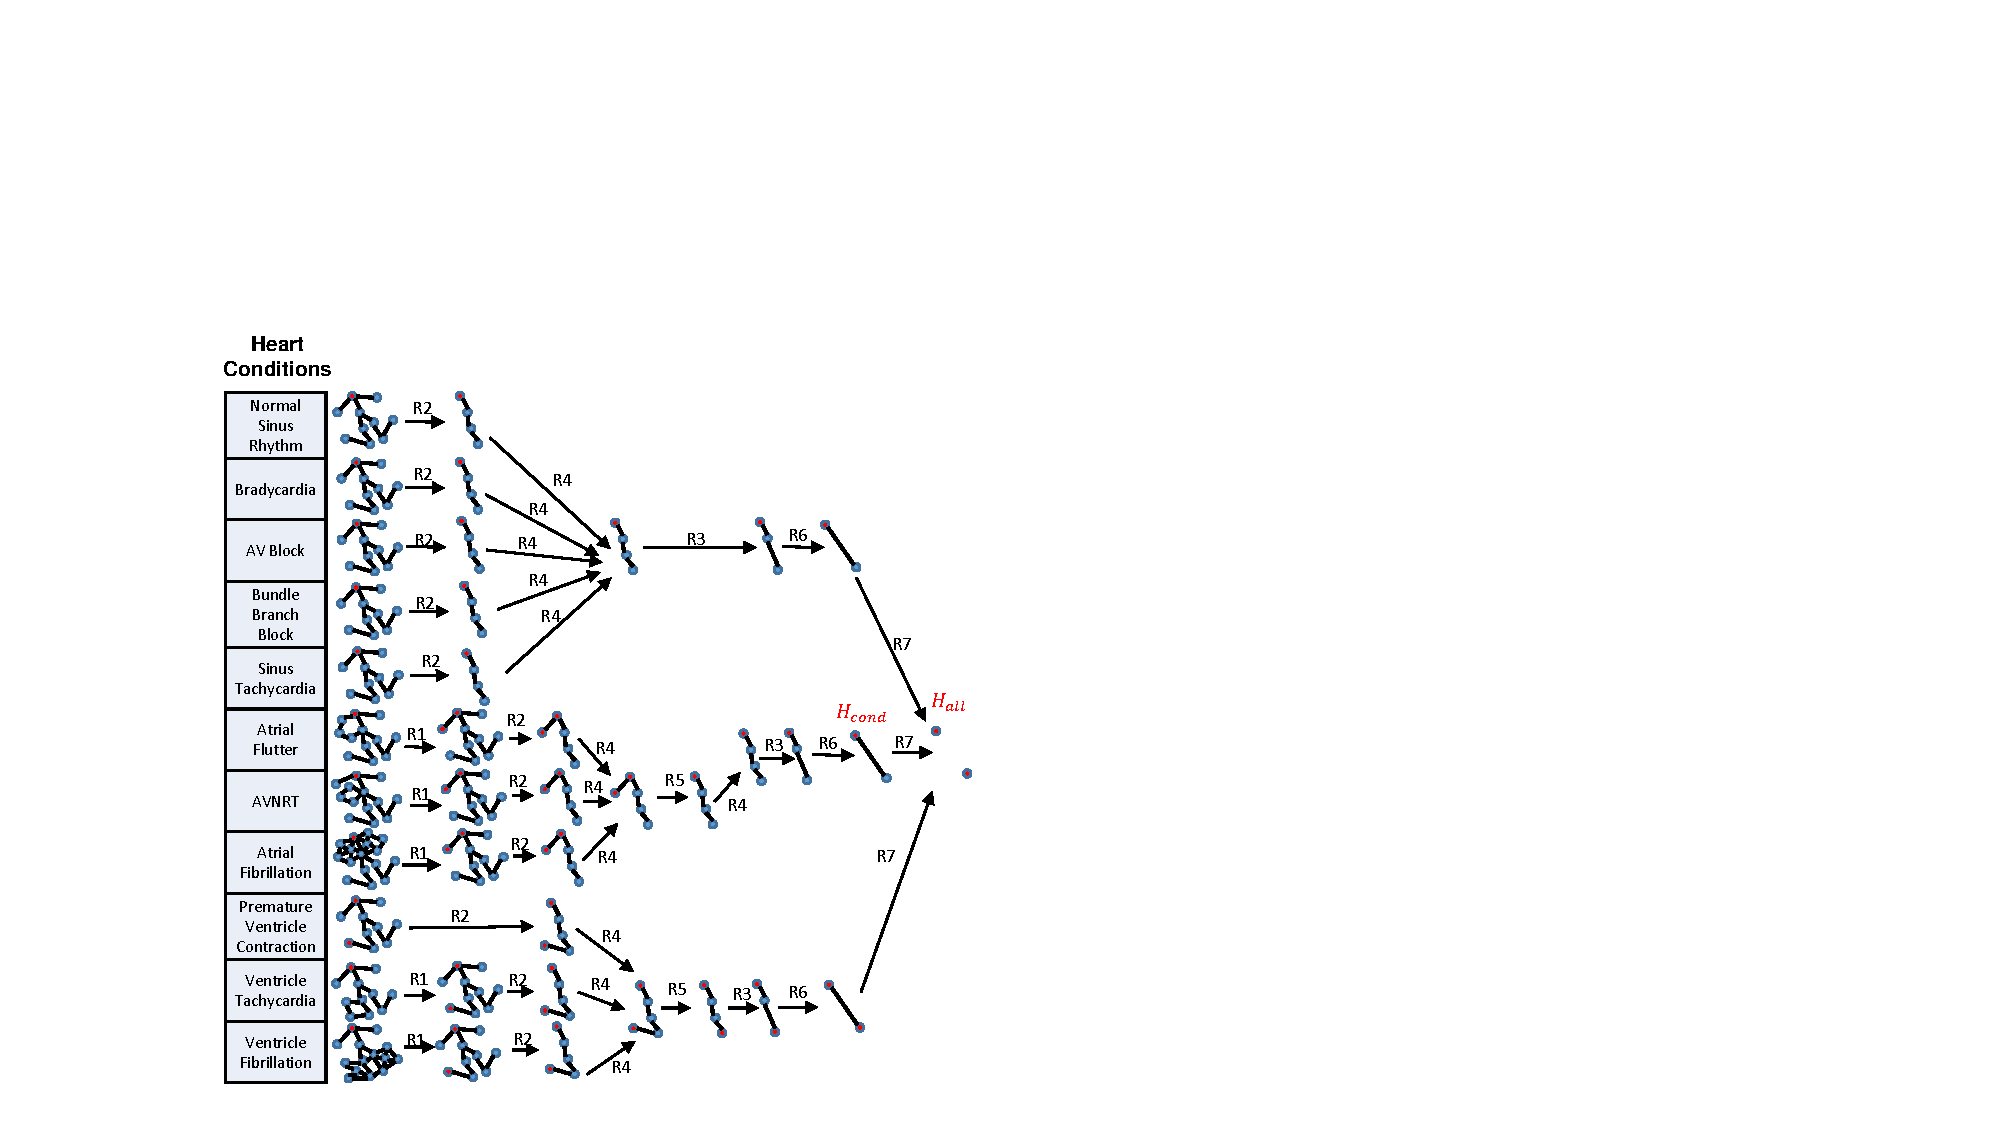
\includegraphics[width=\textwidth]{figs/abs_tree.pdf}
	\caption{\small Multi-scale modeling of the heart. The heart model at a higher level (further to the right) contains all possible inputs to the pacemaker from the heart models at previous levels}
	\label{fig:abs_tree}
\end{figure}



\section{From Verified Models to Verified Code}
During model checking, the abstract model of the pacemaker is verified against safety requirements. The abstract pacemaker model is then automatically synthesized into simulation models and into a code implementation (\figref{modelbaseddesign}) using the UPP2SF model translation tool we developed. 
Each automaton in a network of timed automata is mapped to a parallel state (called parent state) in Stateflow and each location in the automaton is mapped to an exclusive state within the parent state.
Along with mapping all the edges in the UPPAAL model to the Stateflow model, the behaviors of the Stateflow model is a subset of the corresponding UPPAAL model, thus properties verified in the UPPAAL model still hold in the Stateflow model.
This automatic synthesis provides rigorous traceability throughout the development process and ensures that the verified model is translated into verified code using the Stateflow model of the pacemaker with the Simulink embedded coder. 
Similarly the heart model is translated from timed automata to Simulink and also synthesized into a Heart-on-a-Chip for platform level testing.
%% In the semiconductor industry, the Verilog version of a chip design is model checked and automatically synthesized into a logic gate implementation. 

\begin{figure}[t]
	\centering
	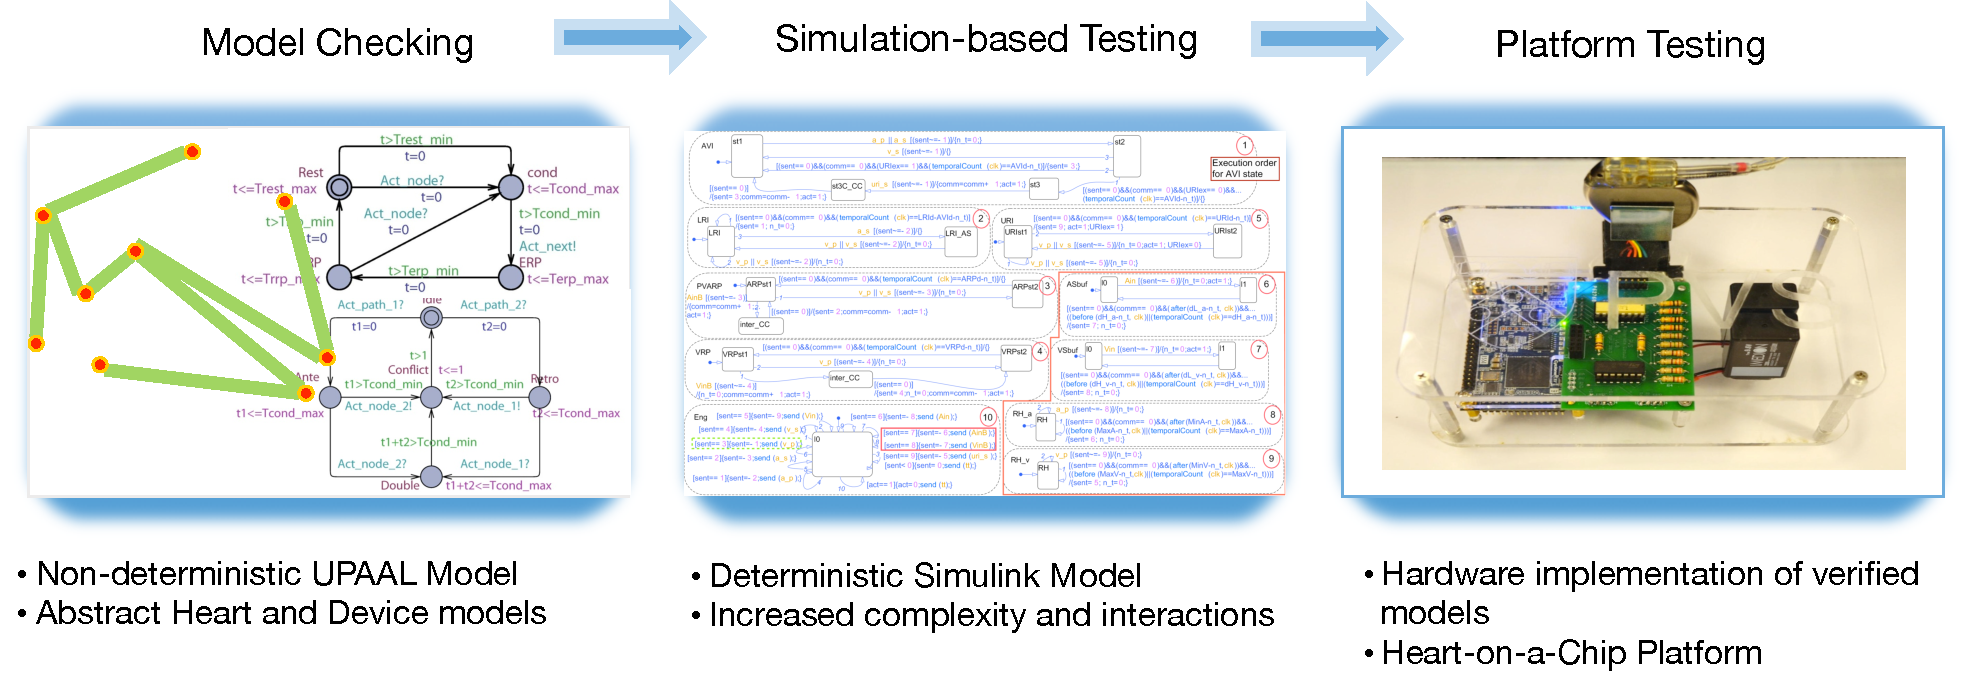
\includegraphics[width=\textwidth]{figs/fig4designtoimplementation.pdf}
	\caption{\small Model translation framework. The pacemaker design is verified using model checking and automatically translated into code implementation. Heart models are available at all levels}
	\label{fig:modelbaseddesign}
\end{figure}
\section{Model-Based Clinical Trials}
The final step before the introduction of a new high-risk medical device to market is the \emph{clinical trial}.
The \emph{randomized controlled trial} (RCT) is the ``gold standard'' for guaranteeing that a medical intervention is safe and efficacious \cite{FriedmanFD10_ClinicalTrials}.
It is in general a major effort involving patients, medical investigators, biostatisticians, ethics boards,  regulators and companies, costing several millions of dollars and running for 4-6 years on average.
Yet technical errors can arise at almost every step of the trial planning, jeopardizing the validity of the results. 
Even if the trial is well-planned, poor execution, unexpected events or even just pure chance can lead to the wrong conclusions.
The applications of computer models to the medical domain presented above have largely centered on the design and verification of a given device, and have mostly eschewed matters related to the clinical trial.
There is however now an opportunity to use these computer models to assist in the planning and conduct of RCTs, as will be presented in this section.
(Another application of modeling to trials is the UVA/PADOVA diabetes model, which replaces \emph{animal} trials for evaluating diabetes control algorithms \cite{pancreas_paul}). 

Suppose that a manufacturer of medical devices is designing a new implantable defibrillator for the treatment of certain abnormal cardiac rhythms, or \emph{arrhythmias}.  
Both the hardware and software are tested by the company to ensure they satisfy their specifications.
The device may then be implanted and tested on animals. 
But up to this point, the effect of the device on humans has not been observed. 
%Observations of interest extend beyond whether the device operates as intended or not to whether it can be implanted safely, whether it has unexpected side effects, and whether it treats the targeted arrhythmias better than current medical care.
The RCT compares the efficacy and safety of the device on two groups of patients: the \emph{treatment group} which is implanted with the new investigational device, and the \emph{control group} which is on standard medical care, e.g. one or more devices already on the market~\cite{FriedmanFD10_ClinicalTrials}.
%The assignment of a patient to the treatment or control group is done \emph{at random}, which guarantees the validity of the statistical tests used to analyze the results and helps ensure that the two groups are comparable.
Both treatment and control groups are monitored for a pre-determined amount of time, at the end of which the rate of treated arrhythmias is evaluated in each group. The results are analyzed to determine whether the difference in rates between the groups, if any, is \emph{significant}, i.e. is unlikely to be due to chance alone.

%We call this the Model-Based Clinical Trial (MBCT). 
%Broadly speaking, we define an MBCT to be a trial in which the subjects are \emph{computer models of the physiological phenomena being studied, including the effect of the device}, rather than humans. 
%An MBCT allows us to run very large-scale targeted simulated trials to better inform our conduct of an actual RCT. 


We can design a \emph{Model-Based Clinical Trial} (MBCT) to test a number of assumptions made by the trial investigators, before the trial starts (Fig.~\ref{fig:mbct}).
In an MBCT, we start by modeling the physiological phenomenon of interest, in this case the spread of electrical activity in the human heart.
The model should be valid of course (i.e., not produce too many non-physiological signals).
For an MBCT the model must also be \emph{rich}: it should be capable of simulating a large variety of arrhythmias that are targeted by the new defibrillator.
Once such a parametrized model is created, we can generate a large number of model instances by sampling the parameter space from appropriate distributions, which may be inferred from previous trials' data.
This constitutes our synthetic cohort. 



We can now analyze the effect of the device in ways not possible or impractical with a clinical trial, so as to guide the RCT investigators when designing the trial's protocol.
For example, we may vary the distribution of arrhythmias in our synthetic cohort and analyze how this affects the device's performance. 
This is equivalent to running multiple trials on different populations in which the arrhythmias appear in different proportions.
The investigators can then use these results to confirm or revise their confidence in the superiority of the new device to standard medical care across populations.
We can also study the sensitivity of the trial's outcome to device settings: by running the trial multiple times with the same synthetic cohort but with different device settings every time, we get solid estimates for how different settings affect the MBCT's outcome. 
This in turn can inform the investigators whether they need to correct for different settings when drawing the trial protocol and when analyzing the results.
Further, by breaking down the MBCT results by arrhythmia (or other interesting criteria) the investigators can make informed decisions, before trial start, on which classes of arrhythmias are most or least susceptible to treatment by the device.
This in turn helps refine the eligibility criteria and focus the trial's efforts on certain classes of patients. 

	
This and other experiments possible in an MBCT increase the probability of success of an RCT by providing early, fast and rigorous testing of various assumptions and hypotheses made by the trial investigators.
%\yhl{For example, for a trial on implantable defibrillators, we can study how variations in a patient's physiological parameters, like speed of propagation of the electric current in the heart, affects the safety and efficacy of the device. 
%This provides valuable insight into which patients should be enrolled in the trial (and in whom the device is most efficacious).
%Another application is to get tighter estimates of statistical quantities like effect size needed before the conduct of the trial.
%A poor effect size estimate leads to a poor sample size estimate, with a real risk of the trial not yielding significant results even if there's a true meaningful difference between treatment and control.
%Yet a third application is to test how changing device settings affects the outcome of interest. 
%This is an example of an experiment ideally suited for model-based investigation, since we can connect the same heart models to the device under all settings, which is typically not possible with real patients.}
%
%\yhl{The Model-Based Clinical Trial promises to usher in a new era in clinical trials planning and medical device development in general, where the trial investigators can quickly, cheaply and reliable assess various assumptions, in ways that are not always feasible in a real trial. 
%A key component of an MBCT is the model.}
%We start with a parametrized model of the heart.
%For the model to be interpretable by physicians, it is important that the parameters have physiological significance, e.g., the refractory periods of the AV node.
%Thus physiological ranges for the parameters are known.

\begin{figure}[t]
	\centering
	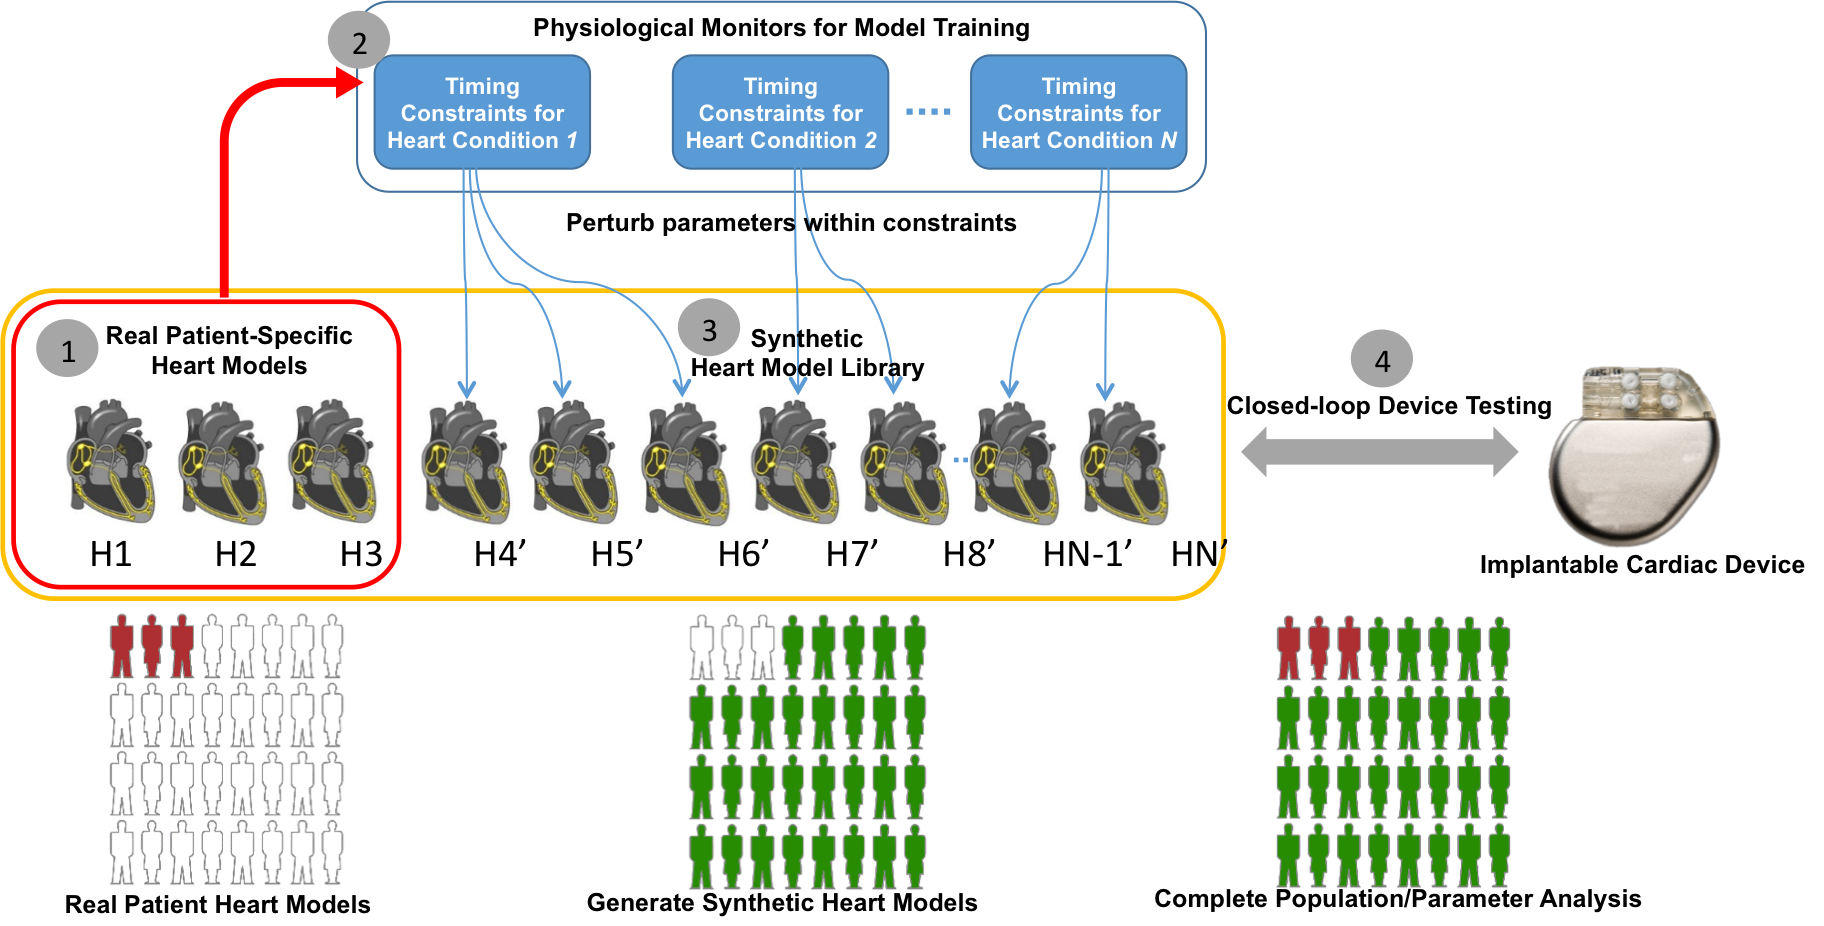
\includegraphics[width=\textwidth]{figs/fig5mbct.png}
	\caption{\small Model-based Clinical Trials. The synthetic cohort is generated by randomizing a parametrized model from an appropriate distribution whose bounds are inferred from clinical data. The parameters are sampled within their physiological ranges, thus generating a large synthetic cohort. Each such model instance is connected to the device and simulated.}
	\label{fig:mbct}
\end{figure}

%Early efforts tying physiological modeling to clinical trials include the UVA/PADOVA diabetes model which is used to generate simulated patients.
%New diabetes control algorithms are evaluated on simulated patients instead of animals to assess their efficacy. These applications of MBCT usher a new era of exciting research challenges for the closed-loop verification, validation and testing medical devices at scale. MBCT have the potential to reduce the scope, cost and probability of failure of clinical trials of medical devices with complex hardware and software. MBCT when viewed as a rapid certification toolchain to speed up medical device approvals is  gaining increasing traction both within the regulatory environment and the medical device industry.
\section{Conclusion}

This article has surveyed the challenges of bringing new medical devices and their software to market from early verification to late-stage clinical trials, and gives an outlook to how modeling and formal methods can play a role in facilitating this process.
\emph{Complexity, limited observability and variability} stand out as three major challenges.
The \emph{complexity} of the physiological phenomena that the device is meant to control stems partially from the multi-scale nature of human physiology, where an organ's operation is affected by both molecular factors and patient's lifestyle.
Moreover, the devices have limited \emph{observability} on these complex physiological phenomena because increased observability usually requires increased invasiveness of the surgical procedures, with all the attending risks.
%Thus, an implantable defibrillator currently has only three contact points with the myocardium, from which it tries to infer the nature of the global electrical activity.
Coupled together, complexity and limited observability imply that the detection and therapy algorithms of devices must deal, safely and reliably, with a lot of uncertainty.
By explicitly allowing for non-determinism in the systems they study, formal methods are well-suited for dealing with uncertainty.
The major challenge for formal methods is the development of appropriate physiological models and abstraction-and-refinement frameworks for addressing the complexity of the phenomena, and abstraction trees take a step in this direction in the domain of electrophysiology.
\emph{Variability} arises as the third major challenge: how to verify that a device works well in a population of patients that varies greatly in its characteristics and medical history?
Clinical trials remain the standard and legally accepted way to answer that question.
While models can not substitute for observations in a human patient, they promise to alleviate the burden of conducting trials by early and rigorous testing of their assumptions.
These applications usher a new era of exciting research challenges at the intersection of computer science, statistics and medicine.

%\section{Conclusion}
\label{sec:conclusion}

Clinical trials study the effect of an intervention \emph{in the patient}, and report patient-level results (e.g., ``The event of interest was observed in X\% of patients in Group 1''). 
Our results are at the condition level: they take the form ``the event of interest was observed in X\% of generated conditions".
To produce patient-level estimates requires an estimate of how conditions are distributed among patients. 
This low-level data is not publicly nor readily available.
A trial's investigators, however, should be able to obtain such data from previous trials.

It is important to stress that in general, one should not expect \emph{absolute numbers} from an MBCT to match those from a clinical trial, nor should this be the goal of the MBCT.
For example, in this work, it is unlikely that our MBCT will yield rates of inappropriate therapy that are equal to the rates obtained by RIGHT itself.
The reasons for this are many:
\begin{itemize}
	\item The RIGHT in vivo cohort, and our synthetic cohort, are not comparable:
	indeed, a myriad of factors affect the outcome of a clinical trial, e.g., whether some patients take up smoking. 
	These factors are not modeled.
	\item The adjudication of episodes in RIGHT (and other trials) is limited by the fact that only therapy episodes were recorded by the devices.
	The adjudication process is further limited by the lack of surface EKGs, which makes it hard to reliably distinguish certain atrial arrhythmias. 
	Neither of these is a limitation in MBCT since we have the ground truth: we know exactly what arrhythmia is being simulated by the model.  Furthermore, the AAEL signals have both device electrograms (EGMs) and the corresponding surface EKGs which allow for precise adjudication.  
	\item Experts may disagree on how to adjudicate the more complex episodes, so our classification of episodes from the AAEL database and the classification of the RIGHT investigators have an irreducible discrepancy.
	Again, this will affect the statistics that they and we compute.
\end{itemize}

That said, we can expect that a good heart model will reveal \emph{the trend} of the results, such as improvement of intervention over control or not, as shown in this paper. 
The MBCT conducted here clearly showed that the Medtronic algorithms outperforms the Boston Scientific's and resulted in a negative outcome of RIGHT across all population distributions and relevant heart conditions. In hindsight, the Boston Scientific-sponsored RIGHT would have needed reconsideration prior to running it to prevent a failed outcome.



\bibliographystyle{unsrt}
\bibliography{bibliography}





\end{document}